% Optional snippets only. Require graphicx in the manuscript preamble.
% Paths assume compilation from the repository root. Not inserted into main.tex.
\begin{figure}[htbp]
  \centering
  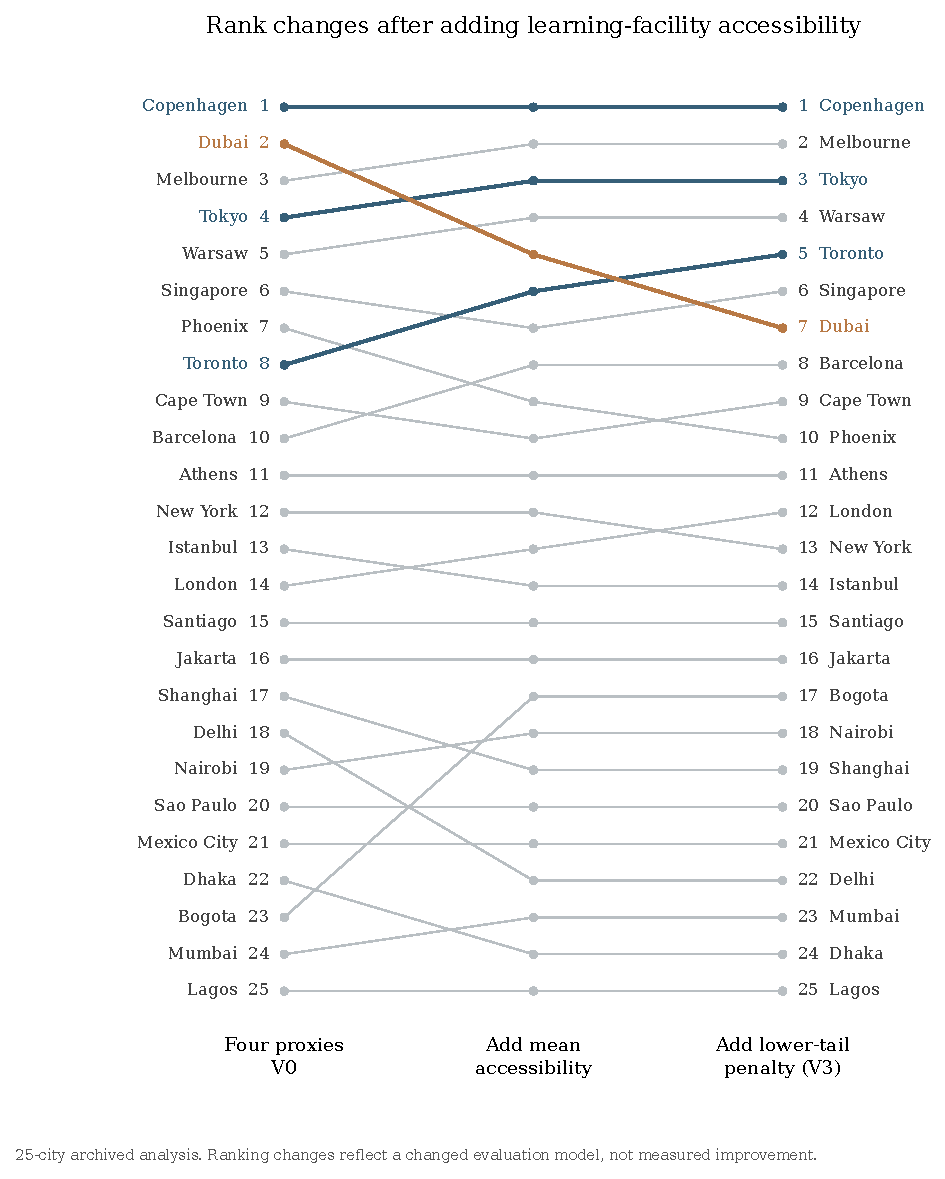
\includegraphics[width=0.88\textwidth]{research/2026-a/visuals/figures/01_rank_revision.pdf}
  \caption{Rank changes in the 25-city sample after adding mean learning-facility accessibility and then a lower-tail adjustment. These are changes in the evaluation model, not changes in observed city conditions.}
  \label{fig:access-rank-revision}
\end{figure}

\begin{figure}[htbp]
  \centering
  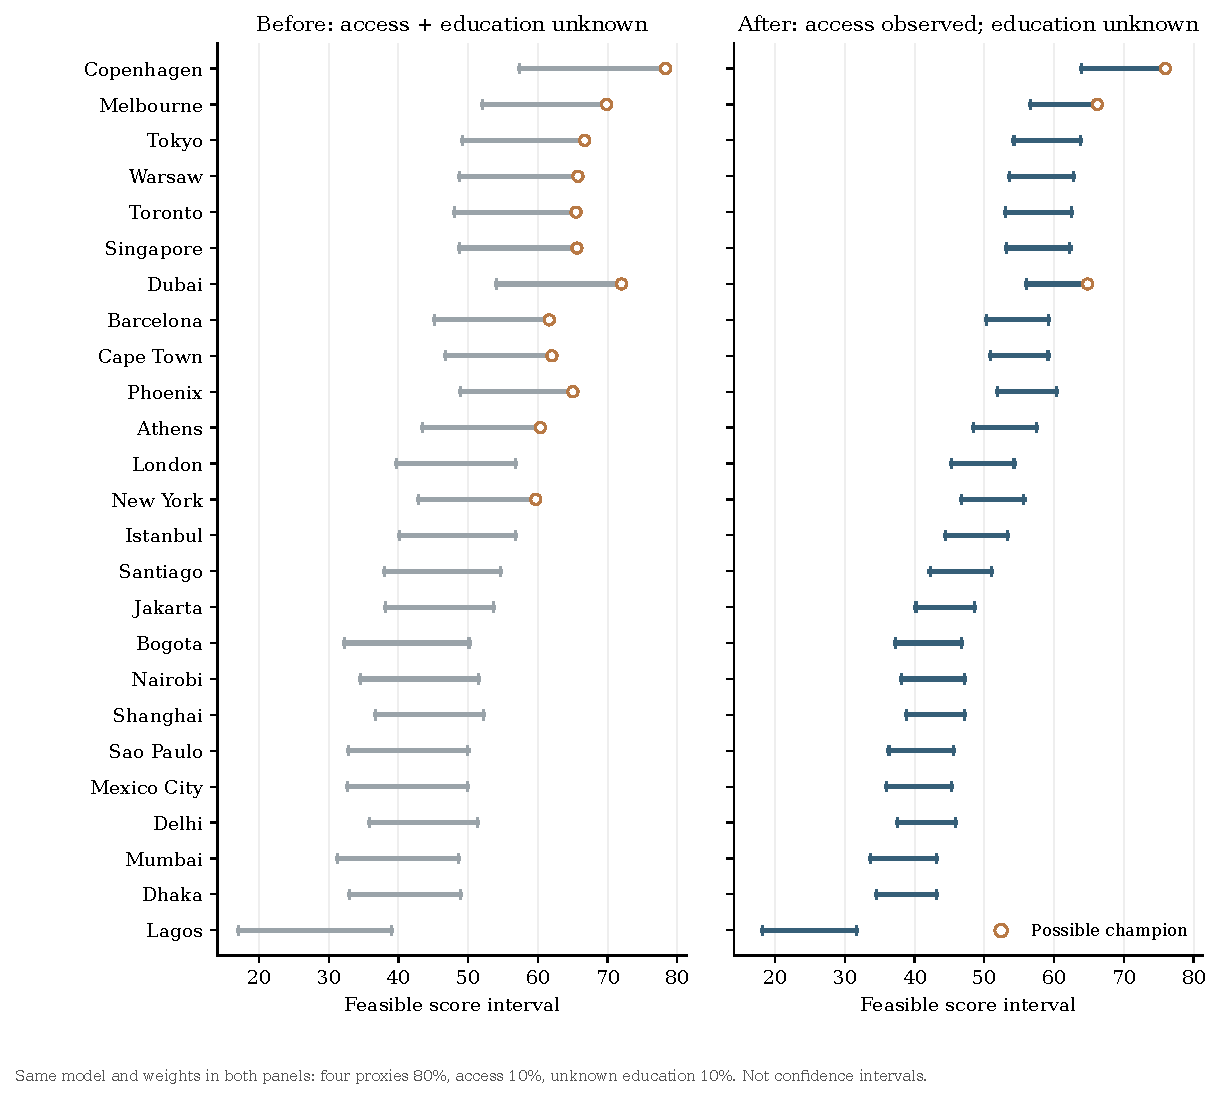
\includegraphics[width=\textwidth]{research/2026-a/visuals/figures/03_information_bounds.pdf}
  \caption{Feasible score intervals before and after observing the accessibility proxy, holding the model and weights fixed. Four baseline proxies receive 80\% total weight, accessibility 10\%, and the unobserved education dimension 10\%. Circles identify possible champions; the intervals are not confidence intervals.}
  \label{fig:access-information-bounds}
\end{figure}
